The storage station is a shelf with ten drawers. The drawers of the shelf can be automatically opened and closed by the
handling robot. It is a mechanical system which is used to store final bent sheet metal parts.

\begin{figure}[h]
    \centering
    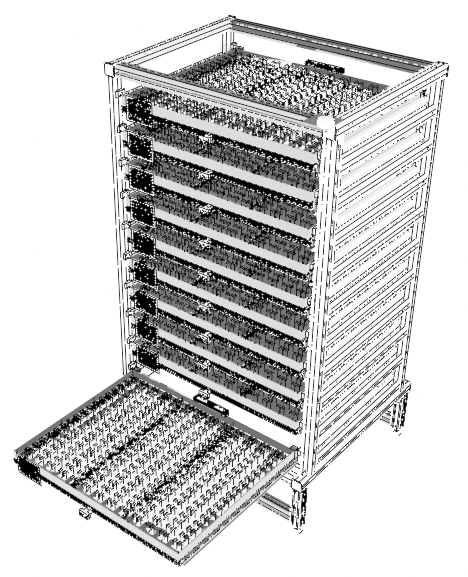
\includegraphics[width=0.3\textwidth]{figures/storage-station-blender.png}
    \caption{Storage Station asset in simulation}
    \label{fig:storage-station}
\end{figure}

When the storage station is full, human operators are to replace a filled shelf with a new empty shelf with a forklift. Thus, this is the only station
which is not fixed in the robotic workcell. The robotic camera mounted on the handling robot needs to determine the correct position of the storage station
after each restart.